\section{Problem Setup}
\label{sec:problem_setup}

\noindent\textbf{Network and records.}
The Central Pollution Control Board publishes hourly PM\(_{2.5}\) and wind for the New
Delhi regulatory monitors \citep{cpcb,cpcb_portal}.  We use
the records from 1 May 2018 to 31 October 2020 at 32 locations, with the two co-located
Pusa monitors averaged and no readings at East Arjun Nagar.  At the 31 locations with
readings, \(93.4\%\) of hourly PM\(_{2.5}\), \(77.3\%\) of wind-direction and \(75.1\%\) of
wind-speed entries are present, and three locations record no wind.  PM\(_{2.5}\) is never
imputed.  Wind is converted from the direction it comes
from to the direction of transport and interpolated with a normalized Gaussian
kernel onto a \(40\times40\) grid that spans the bounding box of the sensor locations
(Appendix~\ref{app:application}).

\noindent\textbf{Source groups.}
Four source groups are declared from proxy maps (Figure~\ref{fig:platform}): brick
kilns and industries from a
regional emissions inventory \citep{GUTTIKUNDA2013101}, population density from a
gridded population product \citep{ColumbiaUniversity2018}, and traffic from a
road-network map \citep{google_maps}.  Each inventory map is cropped to a fixed \(40\times40\)
window of its \(80\times80\) grid, whose alignment with the sensor bounding box is not
verified (Appendix~\ref{app:platform_details}), and divided by its own 99th percentile,
and the traffic map is the mean of four time-of-day road maps normalized this way (the
06:00 map in the inventory is zero).  The activity of group \(k\) is
\(\theta_k(t)=\sum_b c_{kb}\phi_b(t)\) with \(c_{kb}\ge0\) and declared nonnegative
temporal basis functions \(\phi_b\): alternating 12-hour blocks for brick kilns,
one component for industries with a continuous level and higher daytime (07--19 h)
activity, peaks at 07, 13 and 19 h
for population, and time-of-day slots at 00, 06, 12 and 18 h for traffic.  A component is
a pair \(j=(k,b)\).  Each group uses only its own basis functions, so the coefficients of the others, the
set \(\mathcal F_0\), are set to zero before fitting, and no coefficient is removed after
fitting because its estimate is small.  \(J\) is the number of remaining components.
Because each proxy map has its own normalization, the coefficients are in normalized
proxy units, whereas the group signals defined below are in
\(\mu\mathrm g/\mathrm m^3\) and do not depend on that normalization.

\begin{figure}[t]
\centering
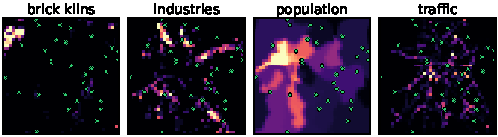
\includegraphics[width=\columnwidth]{figures/fig_platform.pdf}
\caption{Proxy maps of the four source groups on the \(40\times40\) grid (each
inventory map divided by its own 99th percentile, with colour clipped at \(1\)) and the 32
regulatory sensor cells (green).  Traffic is the mean of the four time-of-day road
maps.}
\label{fig:platform}
\end{figure}

\noindent\textbf{Transport operator.}
Emissions released at hour \(t-\ell\) reach the sensors at hour \(t\) after transport
by the wind between the two hours.  Let \(G_{t,t-\ell}\) map emissions on the source
grid at \(t-\ell\) to concentrations at the \(m\) sensors at \(t\) under an
open-boundary Gaussian-puff model driven by the gridded wind \(\omega\) (mass that
leaves the domain is removed), and let \(\mathbf s_k\) be the proxy map of group \(k\).
The PM\(_{2.5}\) that one unit of \(c_{kb}\) produces at the sensors at hour \(t\) is
\begin{equation}
\mathbf a_{t,kb}(\omega)=\sum_{\ell=0}^{\min(L,t-1)}\phi_b(t-\ell)\,G_{t,t-\ell}\,\mathbf s_k
\in\mathbb R^m.
\label{eq:transport_column}
\end{equation}
In \(G_{t,t-\ell}\), a unit release is advected along the interpolated wind and spread by
a Gaussian kernel, evaluated at the sensors, whose variances along and across the mean
wind grow as \(0.7^2\) and \(0.25^2\) square cells per hour of travel.  The model is
two-dimensional and treats PM\(_{2.5}\) as a passive primary tracer, without mixing
height, deposition or secondary formation (Appendix~\ref{app:transport_response}).  Stacking over
hours gives column \(\mathbf a_{kb}(\omega)\) of the operator \(A(\omega)\).  The lag is declared before fitting: \(L=12\) hours in every reported run except the lag
sweep of Experiment 7.

\noindent\textbf{Model, nuisance and projection.}
Let \(\mathbf y\in\mathbb R^N\) stack the observed hourly readings; rows with a missing
reading are removed from \(\mathbf y\), \(A(\omega)\) and \(Q\) alike.  The model is
\begin{equation}
\mathbf y = A(\omega)\,\mathbf c + Q\boldsymbol\gamma + \boldsymbol\epsilon,
\qquad \mathbf c\ge 0,
\label{eq:general_model}
\end{equation}
with \(\mathbf c\in\mathbb R_+^J\), free nuisance coefficients \(\boldsymbol\gamma\) and
noise \(\boldsymbol\epsilon\).  The nuisance basis \(Q\in\mathbb R^{N\times r}\) represents
regional background and smooth trends.  Except in the nuisance-basis variations of Experiments 3 and 11, it
has rank \(r=4\): a constant, a linear time trend and one daily sine--cosine pair,
declared before fitting and never built from the inventories or from fitted
signals.  With
\(P_Q^\perp=I-QQ^\dagger\), the projected problem is
\begin{equation}
\yt=\At\mathbf c+\widetilde{\boldsymbol\epsilon},\qquad
\yt=P_Q^\perp\mathbf y,\qquad
\At=P_Q^\perp A(\omega).
\label{eq:projected_model}
\end{equation}
The projected column \(\at_j=P_Q^\perp\mathbf a_j\), the \emph{fingerprint} of component
\(j\), is the part of its signal that the nuisance cannot reproduce, and because the
projection can absorb a signal, every diagnostic is computed from \(\At\).

\noindent\textbf{The attribution problem.}
Let \(E=\{1,\dots,J\}\) index the components and let \(\mathcal D\) be the declared
partition of \(E\) into source groups.  For \(g\subseteq E\), \(\At_g\) is the submatrix
of the columns in \(g\), and the \emph{signal} of \(g\) is \(\At_g\mathbf c_g\), its
contribution to the projected readings.  It is in \(\mu\mathrm g/\mathrm m^3\) and does
not change when a proxy map is rescaled; a sum of coefficients \(\sum_{j\in g}c_j\) has
neither property.  The task is to choose a partition \(\mathcal P\) of \(E\) whose blocks
are unions of blocks of \(\mathcal D\), using only \(\At\), \(\mathcal D\) and a declared
noise level, before the readings are fitted, and then to report for each block \(g\) its
fitted signal \(\At_g\widehat{\mathbf c}_g\), its share
\(\|\At_g\widehat{\mathbf c}_g\|_1/\sum_{h\in\mathcal P}\|\At_h\widehat{\mathbf c}_h\|_1\), and
the uncertainty of both.  The partition must meet two requirements.  (R1) \emph{Identifiability:} without
noise, the readings determine the signal of every block.  (R2) \emph{Reportability:} at
the declared noise level, the error of every block's fitted signal is bounded by a
stated multiple of the noise.  R1 excludes splits that no amount of data resolves, while R2 excludes splits that the
noise does not allow.  Section~\ref{sec:method} gives the procedure and
Section~\ref{sec:identifiability_theory} the conditions under which it meets both.
